% Mestre em LaTeX - v0.5
% Copyleft 2008-2013 Bruno C. Vellutini - http://organelas.com/
%
% Permission is hereby granted, free of charge, to any person obtaining a copy
% of this software and associated documentation files (the "Software"), to deal
% in the Software without restriction, including without limitation the rights
% to use, copy, modify, merge, publish, distribute, sublicense, and/or sell
% copies of the Software, and to permit persons to whom the Software is
% furnished to do so, subject to the following conditions:
%
% THE SOFTWARE IS PROVIDED "AS IS", WITHOUT WARRANTY OF ANY KIND, EXPRESS OR
% IMPLIED, INCLUDING BUT NOT LIMITED TO THE WARRANTIES OF MERCHANTABILITY,
% FITNESS FOR A PARTICULAR PURPOSE AND NONINFRINGEMENT. IN NO EVENT SHALL THE
% AUTHORS OR COPYRIGHT HOLDERS BE LIABLE FOR ANY CLAIM, DAMAGES OR OTHER
% LIABILITY, WHETHER IN AN ACTION OF CONTRACT, TORT OR OTHERWISE, ARISING FROM,
% OUT OF OR IN CONNECTION WITH THE SOFTWARE OR THE USE OR OTHER DEALINGS IN
% THE SOFTWARE.
%
% Ou seja, utilize e modifique os arquivos como desejar.
% 
% Para mais informações visite http://nelas.github.com/mestre-em-latex/

% Classe do documento
\documentclass[twoside,a4paper,11pt]{report}


% Pacotes e comandos customizados
%%% Pacotes utilizados %%%

%% Codificação e formatação básica do LaTeX
% Suporte para português (hifenação e caracteres especiais)
\usepackage[english,brazilian]{babel}

% Codificação do arquivo
\usepackage[utf8]{inputenx}

% Mapear caracteres especiais no PDF
\usepackage{cmap} 

% Codificação da fonte
\usepackage[T1]{fontenc}
% Usa a lmodern por padrão (caso cm-super não esteja instalada).
\usepackage{lmodern}

%% Microtipografia
% Utiliza recursos como espaçamento entre letras e entre linhas
\usepackage{microtype}
% Habilita protrusão e expansão, ignorando
% compatibilidade (ver documentação do pacote)
\microtypesetup{activate={true,nocompatibility}}
% factor=1100 aumenta a protrusão (default 1000)
% stretch=10 diminui o valor máximo de expansão (default 20)
% shrink=10 diminui o valor máximo de encolhimento (default 20)
\microtypesetup{factor=1100, stretch=10, shrink=10}
% Tracking, espaçamento entre palavras, kerning
\microtypesetup{tracking=true, spacing=true, kerning=true}
% Remover tracking para Small Caps
\SetTracking{encoding={T1}, shape=sc}{0}
% Remove ligaduras para o 'f'. Se necessário, adicionar letras
% separadas por vírgulas
\DisableLigatures[f]{encoding={T1}}
% Documento em versão "final", suporte para outros idiomas
\microtypesetup{final, babel}

% Essencial para colocar funções e outros símbolos matemáticos
\usepackage{amsmath,amssymb,amsfonts,textcomp}

%% Layout
% Customização do layout da página, margens espelhadas
\usepackage[twoside]{geometry}
% Aumenta as margens internas para espiral
\geometry{bindingoffset=10pt}
% Só pra ajustar o layout
\setlength{\marginparwidth}{90pt}
%\usepackage{layout}

% Para definir espaçamento entre as linhas
\usepackage{setspace} 

% Espaçamento do texto para o frame
\setlength{\fboxsep}{1em}

% Faz com que as margens tenham o mesmo tamanho horizontalmente
%\geometry{hcentering}

%% Elementos Gráficos
% Para incluir figuras (pacote extendido)
\usepackage[]{graphicx} 

%% Suporte a cores
\usepackage{color}
% Os argumentos declaram nomes novos, como Cyan e Crimson
% (ver documentação do pacote).
\usepackage[usenames,dvipsnames,svgnames]{xcolor}

% Criar figura dividida em subfiguras
\usepackage{subfig}
\captionsetup[subfigure]{style=default, margin=0pt, parskip=0pt, hangindent=0pt, indention=0pt, singlelinecheck=true, labelformat=parens, labelsep=space}

% Caso queira guardar as figuras em uma pasta separada
% (descomente e) defina o caminho para o diretório:
%\graphicspath{{./figuras/}}

% Customizar as legendas de figuras e tabelas
\usepackage{caption}

% Criar ambientes com 2 ou mais colunas
\usepackage{multicol}

% Ative o comando abaixo se quiser colocar figuras de fundo (e.g., capa)
%\usepackage{wallpaper}
% Exemplo para inserir a figura na capa está no arquivo pre.tex (linha 7)
% Ajuste da posição da figura no eixo Y
%\addtolength{\wpYoffset}{-140pt}
% Ajuste da posição da figura no eixo X
%\addtolength{\wpXoffset}{36pt}

%% Tabelas
% Elementos extras para formatação de tabelas
\usepackage{array}

% Tabelas com qualidade de publicação
\usepackage{booktabs}

% Para criar tabelas maiores que uma página
\usepackage{longtable}

% adicionar tabelas e figuras como landscape
\usepackage{lscape}

%% Lista de Abreviações
% Cria lista de abreviações
\usepackage[notintoc,portuguese]{nomencl}
\makenomenclature

%% Notas de rodapé
% Lidar com notas de rodapé em diversas situações
\usepackage{footnote}

% Notas criadas nas tabelas ficam no fim das tabelas
\makesavenoteenv{tabular}

% Conta o número de páginas
\usepackage{lastpage}

%% Referências bibliográficas e afins
% Formatar as citações no texto e a lista de referências
%\usepackage{natbib}
\usepackage[authoryear,round,longnamesfirst]{natbib}
% Adicionar bibliografia, índice e conteúdo na Tabela de conteúdo
% Não inclui lista de tabelas e figuras no índice
\usepackage[nottoc,notlof,notlot]{tocbibind}

%% Pontuação e unidades
% Posicionar inteligentemente a vírgula como separador decimal
\usepackage{icomma}

% Formatar as unidades com as distâncias corretas
\usepackage[tight]{units}

%% Cabeçalho e rodapé
% Controlar os cabeçalhos e rodapés
\usepackage{fancyhdr}
% Usar os estilos do pacote fancyhdr
\pagestyle{fancy}
\fancypagestyle{plain}{\fancyhf{}}
% Limpar os campos do cabeçalho atual
\fancyhead{}
% Número da página do lado esquerdo [L] nas páginas ímpares [O] e do lado direito [R] nas páginas pares [E]
\fancyhead[LO,RE]{\thepage}
% Nome da seção do lado direito em páginas ímpares
\fancyhead[RO]{\nouppercase{\rightmark}}
% Nome do capítulo do lado esquerdo em páginas pares
\fancyhead[LE]{\nouppercase{\leftmark}}
% Limpar os campos do rodapé
\fancyfoot{}
% Omitir linha de separação entre cabeçalho e conteúdo
\renewcommand{\headrulewidth}{0pt}
% Omitir linha de separação entre rodapé e conteúdo
\renewcommand{\footrulewidth}{0pt}
% Altura do cabeçalho
\headheight 15pt

% Dados do projeto
\newcommand{\nomedoaluno}{Hudson Chaves Costa}
\newcommand{\titulo}{Três Ensaios em Comportamento dos Preços na Economia Brasileira}

%% Links dinâmicos
% Suporte para hipertexto, links para referências e figuras
\usepackage{hyperref}
% Configurações dos links e metatags do PDF a ser gerado
\hypersetup{colorlinks=true, linkcolor=blue, citecolor=blue, filecolor=blue, pagecolor=blue, urlcolor=green,
            pdfauthor={\nomedoaluno},
            pdftitle={\titulo},
            pdfsubject={Assunto do Projeto},
            pdfkeywords={palavra-chave, palavra-chave, palavra-chave},
            pdfproducer={LaTeX},
            pdfcreator={pdfTeX}}

%% Inserir comentários no texto
% Marcar mudanças e fazer comentários
%\usepackage[margins]{trackchanges}
% Iniciais do autor
%\renewcommand{\initialsTwo}{bcv}
% Notas na margem interna
%\reversemarginpar

%% Comandos customizados

% Espécie e abreviação
\newcommand{\subde}{\emph{Clypeaster subdepressus}}
\newcommand{\subsus}{\emph{C.~subdepressus}}

%% Pacotes não implementados
% Para não sobrar espaços em branco estranhos
%\widowpenalty=1000
%\clubpenalty=1000

% Início do texto
\usepackage{Sweave}
\begin{document}
\Sconcordance{concordance:mestrado.tex:mestrado.Rnw:%
1 26 1}
\Sconcordance{concordance:mestrado.tex:./meta.Rnw:ofs 27:%
1 189 1}
\Sconcordance{concordance:mestrado.tex:mestrado.Rnw:ofs 217:%
29 2 1 1 0 1 1}
\Sconcordance{concordance:mestrado.tex:./pre.Rnw:ofs 222:%
1 217 1}
\Sconcordance{concordance:mestrado.tex:./cap1.Rnw:ofs 440:%
1 41 1}
\Sconcordance{concordance:mestrado.tex:./cap2.Rnw:ofs 482:%
1 206 1}
\Sconcordance{concordance:mestrado.tex:./final.Rnw:ofs 689:%
1 6 1}
\Sconcordance{concordance:mestrado.tex:mestrado.Rnw:ofs 696:%
37 7 1}
\Sconcordance{concordance:mestrado.tex:./apendice.Rnw:ofs 704:%
1 4 1}
\Sconcordance{concordance:mestrado.tex:mestrado.Rnw:ofs 709:%
46 2 1}

% Limpa cabeçalhos.
% (solução para lidar com a númeração das páginas pré-textuais).
\pagestyle{empty}

%% Capa
\begin{titlepage}

% Se quiser uma figura de fundo na capa ative o pacote wallpaper
% e descomente a linha abaixo.
% \ThisCenterWallPaper{0.8}{nomedafigura}

\begin{center}
{\LARGE \nomedoaluno}
\par
\vspace{200pt}
{\Huge \titulo}
\par
\vfill
\textbf{{\large Porto Alegre}\\
{\large \the\year}}
\end{center}
\end{titlepage}

% Faz com que a página seguinte sempre seja ímpar (insere pg em branco)
\cleardoublepage

% Numeração em elementos pré-textuais é opcional (ativada por padrão).
% Para desativá-la comente a linha abaixo.
%\pagestyle{fancy}

% Números das páginas em algarismos romanos
\pagenumbering{roman}

%% Página de Rosto

% Numeração não deve aparecer na página de rosto.
\thispagestyle{empty}

\begin{center}
{\LARGE \nomedoaluno}
\par
\vspace{200pt}
{\Huge \titulo}
\end{center}
\par
\vspace{90pt}
\hspace*{175pt}\parbox{7.6cm}{{\large Projeto de Tese apresentado ao Programa de Pós-Graduação em Economia da Universidade Federal do Rio Grande do Sul na Área de Economia Aplicada.}}

\par
\vspace{1em}
\hspace*{175pt}\parbox{7.6cm}{{\large Orientador: Prof. Dr. Sabino Porto da Silva Júnior}}

\par
\vfill
\begin{center}
\textbf{{\large Porto Alegre}\\
{\large \the\year}}
\end{center}

\newpage

% Ficha Catalográfica
%\hspace{8em}\fbox{\begin{minipage}{10cm}
%Aluno, Nome C.

%\hspace{2em}\titulo

%\hspace{2em}\pageref{LastPage} páginas

%\hspace{2em}Dissertação (Mestrado) - Instituto de Biociências da Universidade de São Paulo. Departamento de XXXXXXXX.

%\begin{enumerate}
%\item Palavra-chave
%\item Palavra-chave
%\item Palavra-chave
%\end{enumerate}
%I. Universidade de São Paulo. Instituto de Biociências. Departamento de XXXXXXXX.

%\end{minipage}}
%\par
%\vspace{2em}
%\begin{center}
%{\LARGE\textbf{Comissão Julgadora:}}

%\par
%\vspace{10em}
%\begin{tabular*}{\textwidth}{@{\extracolsep{\fill}}l l}
%\rule{16em}{1px}   & \rule{16em}{1px} \\
%Prof. Dr. 		& Prof. Dr. \\
%Nome			& Nome
%\end{tabular*}

%\par
%\vspace{10em}

%\parbox{16em}{\rule{16em}{1px} \\
%Prof. Dr. \\
%Nome do Orientador}
%\end{center}

%\newpage

% Dedicatória
% Posição do texto na página
%\vspace*{0.75\textheight}
%\begin{flushright}
  %\emph{Dedicatória...}
%\end{flushright}

%\newpage

% Epígrafe
%\vspace*{0.4\textheight}
%\noindent{\LARGE\textbf{Exemplo de epígrafe}}
% Tudo que você escreve no verbatim é renderizado literalmente (comandos não são interpretados e os espaços são respeitados)
%\begin{verbatim}
%O que é bonito?
%É o que persegue o infinito;
%Mas eu não sou
%Eu não sou, não…
%Eu gosto é do inacabado,
%O imperfeito, o estragado, o que dançou
%O que dançou…
%Eu quero mais erosão
%Menos granito.
%Namorar o zero e o não,
%Escrever tudo o que desprezo
%E desprezar tudo o que acredito.
%Eu não quero a gravação, não,
%Eu quero o grito.
%Que a gente vai, a gente vai
%E fica a obra,
%Mas eu persigo o que falta
%Não o que sobra.
%Eu quero tudo que dá e passa.
%Quero tudo que se despe,
%Se despede, e despedaça.
%O que é bonito…
%\end{verbatim}
%\begin{flushright}
%Lenine e Bráulio Tavares
%\end{flushright}

%\newpage

% Agradecimentos

% Espaçamento duplo
%\doublespacing

%\noindent{\LARGE\textbf{Agradecimentos}}

%Agradeço ao meu orientador, ao meu co-orientador, aos meus colaboradores, aos técnicos, à seção administrativa, à fundação que liberou verba para minhas pesquisas, aos meus amigos, à minha família e ao meu grande amor.

%\newpage

%\vspace*{10pt}
% Abstract
%\begin{center}
  %\emph{\begin{large}Resumo\end{large}}\label{resumo}
%\vspace{2pt}
%\end{center}
% Pode parecer estranho, mas colocar uma frase por linha ajuda a organizar e reescrever o texto quando necessário.
% Além disso, ajuda se você estiver comparando versões diferentes do mesmo texto.
% Para separar parágrafos utilize uma linha em branco.
%\noindent
%Esta, quem sabe, é a parte mais importante do seu trabalho.
%É o que a maioria das pessoas vai ler (além do título).
%Seja objetivo sem perder conteúdo.
%Um bom resumo explica porquê este trabalho é interessante, relata como foi feito, o que foi encontrado, contextualiza os resultados e delineia conclusões.
%\par
%\vspace{1em}
%\noindent\textbf{Palavras-chave:} palavra1, palavra2, palavra3
%\newpage

% Criei a página do abstract na mão, por isso tem bem mais comandos do que o resumo acima, apesar de serem idênticas.
%\vspace*{10pt}
% Abstract
%\begin{center}
  %\emph{\begin{large}Abstract\end{large}}\label{abstract}
%\vspace{2pt}
%\end{center}

% Selecionar a linguagem acerta os padrões de hifenação diferentes entre inglês e português.
%\selectlanguage{english}
%\noindent
%This is the most important part of your work.
%This is what most people will read.
%Be concise without omitting content.
%A good abstract explains why this is an interesting study, tells how it was done, what was found, contextualizes the results and set conclusions.
%\par
%\vspace{1em}
%\noindent\textbf{Keywords:} word1, word2, word3

% Voltando ao português...
%\selectlanguage{brazilian}

%\newpage

% Desabilitar protrusão para listas e índice
\microtypesetup{protrusion=false}

% Lista de figuras
%\listoffigures

% Lista de tabelas
%\listoftables

% Abreviações
% Para imprimir as abreviações siga as instruções em 
% http://code.google.com/p/mestre-em-latex/wiki/ListaDeAbreviaturas
%\printnomenclature

% Índice
\tableofcontents

% Re-habilita protrusão novamente
\microtypesetup{protrusion=true}
% Faz com que o ínicio do capítulo sempre seja uma página ímpar
\cleardoublepage

% Inclui o cabeçalho definido no meta.tex
\pagestyle{fancy}

% Números das páginas em arábicos
\pagenumbering{arabic}

\chapter{INTRODUÇÃO}\label{intro}

Sabe-se que a Teoria Econômica ortodoxa divide-se em dois grandes grupos: microeconomia e macroeconomia. Para \citet{bresser1968macroeconomia}, a primeira está focada na análise de funcionamento geral da economia por meio do comportamento dos agentes econômicos individuais (consumidores e produtores). Já a segunda, realiza essa mesma análise, partindo do estudo de agregados econômicos, como a renda, o consumo, e o investimento. Segundo \citet{ball1994sticky} existem dois tipos de macreconomistas: os que acreditam que a rigidez de preços tem um papel importante nas flutuações econômicas de curto prazo e os que atribuem a choques tecnológico tais flutuações.

A partir de Keynes, a teoria macroeconômica evoluiu em diversos caminhos. Em 1937 o modelo Hicks-Hansen, considerado uma das principais formulações matemáticas da Teoria Geral do Emprego, dos Juros e da Moeda, atribuiu importante valor à doutrina da preferência pela liquidez e sua interpretação dos efeitos do investimento sobre a renda (multiplicador) e dos efeitos da renda sobre o investimento (acelerador). Contudo, os keynesianos de Cambridge retomaram as ideias neoclássicas por meio de \citet{friedman1992money} que introduziram a versão aceleracionista da curva de Phillips (taxa natural de desemprego e expectativas adaptativas). Além disso, o monetarismo defende que a taxa natural de desemprego é determinada pelas forças de oferta. 

Não obstante, as críticas de \citet{lucas1972expectations} que deram origem à macroeconomia novo-classica, são consideradas como importantes para o pouco sucesso do monetarismo.  Porém, devido às deficiências internas e pela falta de aderência dos modelos à realidade empírica, criticas surgiram sobre a macroeconomia novo-clássica (\citet{mccallum1998stickiness}).

Nos anos 1980, vários autores neoclássicos  questionaram fortemente a teoria Novo-Clássica e elaboraram um retorno ao keynesianismo neoclássico, com a teoria Novo-Keynesiana (\citet{blinder1983money}). Segundo \citet{dathein2000crescimento} em nível microeconômico, a teoria Novo-Keynesiana adota os fundamentos neoclássicos de agentes maximizadores fazendo o melhor uso das informações disponíveis. Em relação aos microfundamentos da macroeconomia, destacam-se as falhas ou barreiras de mercado. Dessa forma, constata-se a existência de falhas de coordenação de forma que decisões individuais podem gerar externalidades macroeconômicas. Por outro lado, no contexto econômico existe concorrência imperfeita, havendo agentes formadores, e não simplesmente tomadores, de preços e salários. Então, para os agentes econômicos, existe rigidez de preços e salários originada por assimetrias de mercado, heterogeneidade de bens e fatores e informações imperfeitas. A competição imperfeita, por outro lado, cria externalidades de demanda agregada que levam a que os custos sociais da rigidez de preços sejam maiores que os custos privados. 

Como é possível observar, há décadas diversas pesquisas teóricas têm focado na fundamentação microeconômica da rigidez de preços, um elemento chave nas explicações dos efeitos reais da política monetária. Por outro lado, a literatura empírica sobre rigidez de preços é pouco encontrada. \citet{bils2004some} fizeram uma importante contribuição ao estudar de forma desagregada dados do \emph{Consumer Price Index} (CPI) dos EUA a partir de 1990 e mostrar que o preço médio mudou uma vez a cada 4,3 meses. Embora outras significantes contribuições seguiram este trabalho, importantes questões empíricas permanecem em grande parte sem resposta.

\citet{cavallo2010scraped} fez questionamentos sobre os fundamentos da rigidez de preços. Entre eles, se as decisões de preço são temporalmente dependentes ou relacionada ao estado econômico subjacente, se a rigidez de preços é realmente conduzida por custo de menu e assimetria de informação, o papel da competição e sincronização dos preços e como o ambiente econômico, experiências passadas de inflação e quadros institucionais influenciam na forma como os preços se ajustam.

A principal restrição para pesquisa empírica é que os dados em nível de produto são limitados em termos de frequência, países e contextos em que eles são coletados. Dados do CPI dos EUA e Europa têm se tornado viáveis para pesquisadores em uma base limitada. Embora esses bancos de dados cubram uma vasta gama de produtos, eles são tipicamente viáveis para países desenvolvidos com ambiente macroeconômico estável, onde choques agregados são leves e os mecanismos relevantes em nível micro com objetivos macro são difíceis de identificar. 

Por fim, dados tradicionais de pesquisas de instituições públicas e privadas não possuem tais características e assim, são limitantes para pesquisas empíricas sobre o impacto de políticas monetárias e rigidez de preços.

O presente projeto de tese propõe a utilização da tecnologia de \emph{web scraping} assim como \citet{cavallo2010scraped} para coletar preços de sites de diversos setores da economia brasileira. Assim, pretende-se contribuir para a pesquisa empírica no mercado brasileiro no que tange à avaliação empírica da rigidez de preços e também gerar um índice de inflação que possa ser considerado proxy para os índices divulgados pelo governo. 

\section*{JUSTIFICATIVA}

Os preços são fundamentais para o funcionamento da economia. São diversas fontes de preços em áreas distintas: bens e serviços, trabalho (salário), dinheiro e tempo (juros), empresas (ações), uma moeda em relação a outra (câmbio). Historicamente, o Brasil sofreu com altas taxas de inflação que prejudicavam o poder de compra da população nos anos 80 e inicio dos anos 90. A partir da estabilização dos preços com o Plano Real, fez-se necessário o acompanhamento do seu comportamento para evitar o retorno às taxas anteriores de inflação. Um dos principais preços da economia é a taxa de júros básicos utilizada pelo Banco Central para o controle da inflação. Tal taxa é aumentada quando há sinal de pressão inflacionária e ciclo de atividade em alta.

Assim, políticas monetárias e fiscais são usadas como forma de manter os preços sob controle e por conseguinte, influenciar o desempenho da economia. A qualidade das informações sobre os preços é um fator importante para que os órgãos públicos possam tomar decisões eficientes no que tange aos objetivos de controle de inflação. Estudos empiricos já mostraram a importância de dados coletados da \emph{web} na avaliação dos pressupostos de rigidez de preços e proposição de medida de inflação oriunda de informações \emph{online}.

O presente projeto de tese apresenta o seguinte problema de pesquisa: preços coletadas diretamente da \emphg{web} produzem índices de inflação que são condizentes com os publicados pelos órgãos públicos brasileiros? Empiricamente, a rigidez de preços pode ser mensudarada e avaliada tanto qualitativamente quanto estatisticamente? É possível avaliar o impacto das políticas públicas sobre os preços em diferentes regiões do país ou até mesmo setores da economia?


\section*{OBJETIVOS}

O objetivo geral deste projeto é avaliar empiricamente a rigidez de preços na economia brasileira, bem como, propor um índice de inflação oriundo de preços coletados da \emph{web}.

Dentro deste escopo, os objetivos específicos são: melhor compreensão do comportamento microeconômico dos preços e suas implicações para a economia. Tal ponto pode ser um fator vital para a construção de políticas públicas mais eficientes tanto em âmbito regional quanto em setores diversos da economia.  
\pagestyle{empty}
\cleardoublepage
\pagestyle{fancy}

\chapter{REVISÃO BIBLIOGRÁFICA}\label{cap2}

Muitos mecanismos microeconômicos têm sido propostos para explicar porque os preços são rígidos. A maior parte deles podem ser amplamente classificados em dois tipos de modelos: tempo-denpendente e estado-denpendente. Nos modelos tempo-denpendentes, o momento de ajustamento nos preços é determinado exogenamente. Uma firma é capaz de definir o preço ótimo depois de um dado número de períodos (conforme \citet{taylor1980aggregate}), ou aleatoriamente em cada período (conforme \citet{calvo1983staggered}). Com ajustamentos aleatórios, mudanças nos preços de qualquer tamanho são possíveis e existem uma fração estável de firmas ajustando em cada período, independentemente de quanto tempo já passou desde a última alteração no preço. 

Modelos estado-dependentes, começam com os modelos de custo de menu de \citet{barro1972theory} e \citet{sheshinski1977inflation} e mais recentemente \citet{dotsey1999state} e \citet{golosov2007menu}, tendem a ter maior fundamentação microeconômica. Eles são baseados na hipótese de que firmas são capazes de mudar seus preços em qualquer momento, mas devem enfrentar custos de ajustamento para fazer isso. Tais custos podem incluir custos trabalhistas para fazer as alterações, custos gerenciais para tomar a decisão, ou mesmo custos de “ira do cliente” como reação do cliente após o ajustamento nos preços. Em modelos estado-dependentes existem algumas pequenas alterações (dado que não vale a pena pagar o custo de menu) e os ajustem tendem a ocorrer mais frequentemente em preços “velhos” (onde o desvio do ótimo é maior).

Como já mencionado anteriormente, pesquisas empíricas que busquem avaliar a rigidez de preços tem pouca audiência em função da dificuldade de acesso a dados de preços de produtos e serviços em uma frequência considerável. O presente projeto de tese tem como objetivo avaliar se dados coletados da nuvem de diversos sites (supermercados, postos de gasolina, farmácias, ...) são capazes de contribuir para o estudo empírico da rigidez de preços. Além disso, propor um índice de inflação que possa ser utilizado como \emph{proxy} para os índices divulgados pelos órgãos públicos e comumente usado no mercado.  

O tema ainda é pouco explorado na academia, mas a difusão da internet e a facilidade de acesso via telefones celulares, por exemplo, são fatores que sinalizam para a importância que as informações armazenadas nas páginas de sites têm para estudos econômicos. 

O \emph{Billion Prices Project} (BPP) no \emph{Massachusetts Institute of Technology} (MIT) é uma iniciativa acadêmica que usa preços coletados diariamente de varejistas com lojas online em todo o mundo para conduzir pesquisa econômica. O projeto tem sido uma fonte de dados para diversas pesquisas acadêmicas no que tange à rigidez de preços, impacto de união monetária nos preços relativos internacionais, taxas de câmbios reais, lei do preço único, inflação online versus inflação oficial de países emergentes onde as medidas divulgadas para esta variável são questionadas pelo mercado, comportamento dos preços e oferta de produtos em desastres naturais como os terremotos do Chile em 2010 e Japão em 2011.

\citet{cavallo2010scraped} apresenta de forma inovadora a utilização de dados diários de preços individuais coletados de páginas de supermercados na Argentina, Brasil, Chile e Colômbia entre outubro de 2007 a outubro de 2008 para a avaliar o comportamento microeconômico dos preços e sua implicação para modelos macroeconômicos. O autor apresenta fatos estilizados sobre a rigidez dos preços nestes quatro países e mostram que a distribuição do tamanho da mudança nos preços é bimodal (com algumas alterações próximas a zero por cento). As funções de risco agregado são inclinadas para cima ou em forma côncava, e existe sincronização de mudanças nos preços para marcas concorrentes. Esses fatores desafiam visões comumente vistas na literatura de rigidez de preços que tem sido influenciada por trabalhos teóricos anteriores. 
  
Além disso, \citet{cavallo2010scraped} providencia um índice de inflação alternativo para a Argentina onde estatísticas oficiais tem se tornado irreal para muitas pessoas. Eles mostraram que a inflação anual era consistentemente duas ou três vezes maior do que o índice oficial divulgado. 

 \citet{cavallo2012currency} utilizaram um conjunto de dados de preços online de bens idênticos vendidos em dezenas de países por quatro dos maiores varejistas globais (Apple, IKEA, H\&M, ZARA) para estudar a taxa de câmbio real e seus comportamentos agregados. Em contraste com a literatura, demonstraram que a lei do preço único (LPU) se matem dentro da zona do euro para dez dos milhares de bens vendidos pelos quatro varejistas em três industrias não relacionadas, implicando taxa de juro real igual a um.

Não obstante, \citet{cavallo2012currency} mostraram que desvios da LPU são significativamente maiores para esses mesmos produtos em países com diferentes moedas, mesmo se sua taxa de câmbio real é indexada. Por exemplo, preços na zona do euro diferem tipicamente daqueles na Suécia, que tem uma taxa de câmbio flutuante e também daqueles na Dinamarca, que vincula sua moeda ao euro. Isto esclarece que a moeda comum por si e não simplesmente a falta de volatilidade nominal, é importante na redução da dispersão dos preços entre países. Além disso, a LPU com os EUA se mantem mais para países dolarizados como Equador e El Salvador do que para países como Hong Kong ou Jordânia, que tem suas próprias moedas, mas vinculadas ao dólar americano. 

\citet{cavallo2013prices}	estudaram o comportamento dos preços diários de supermercados e disponibilidade de produtos seguindo dois desastres naturais recentes: terremoto no Chile em 2010 e terremoto no Japão em 2011. Em ambos os casos existiu um efeito imediato e persistente sobre a disponibilidade de produtos. O número de bens disponíveis para venda caiu 32\% no Chile e 17\% no Japão a partir do dia do desastre para seus pontos mais baixos, que ocorreram 61 e 18 dias depois dos terremotos, respectivamente. A disponibilidade de produtos recuperou lentamente e uma significante parte dos bens permaneceram sem estoque depois de seis meses. Ao contrário, os preços ficaram estáveis por meses até mesmo para os bens que estavam experimentando grave carência. Essas tendências estão presentes para todos os níveis de agregação, mas existe heterogeneidade entre categorias. Ainda, \citet{cavallo2013prices} para a frequência e magnitude nas mudanças de preços em ambos os países e encontraram que os resultados no Chile são consistentes com modelos de precificação onde varejistas tem medo da “ira do cliente”. No Japão a evidência sugere um maior papel para a ruptura de distribuição que restringe a capacidade dos varejistas em distribuir após o terremoto. 

Recentemente, \citet{cavallo2014price} refletiram sobre as implicações de um país aderir a uma área de moeda comum nos preços relativos. Os autores consideraram o caso da Letónia, que recentemente deixou sua taxa de câmbio indexada e se juntou à zona do euro em janeiro de 2014. O artigo é o primeiro a usar dados de alta frequência para demonstrar que aderir a uma união monetária tem implicações econômicas para os preços dos países e a taxa de câmbio real. Tal experimento é particularmente útil porque a entrada da Letónia à zona do euro não carregou consigo profundas mudanças nas políticas governamentais. 

Utilizando preços de milhares de bens vendidos pela Zara (coletados via web scraper), a maior varejista de roupas do mundo, os autores observaram que a dispersão dos preços na Letónia desmoronou rapidamente após a adoção do euro. O percentual de bens com preços quase idênticos em Letónia e Alemanha aumentou de 6\% para 89\%. Por outro lado, a tamanho mediano do preço declinou de 7\% para 0\%. Se um número maior de firmas também se comporta desta maneira, esses resultados sugerem que se tornar membro de uma união monetária tem significante implicações para a taxa de câmbio real de países. 


\pagestyle{empty}
\cleardoublepage
\pagestyle{fancy}

\chapter{METODOLOGIA}\label{cap3}

\section*{WEB SCRAPING}

O surgimento da internet, em particular a Web (\emph{Web Wide Word}) trouxe um crescimento exponencial nas disposições de informações. Embora muitas dessas informações sejam úteis, elas raramente estão de uma forma que podemos utilizá-las, pois ainda é comum pessoas gastarem horas na coleta manual de dados de páginas da web. Especificamente, apesar de disponibilidade, poucos trabalhos acadêmicos em Economia utilizam desta fonte de dados para análise econômica empírica. Tal característica pode ser dada pela dificuldade dos pesquisadores na área em lidar com linguagem de programação que demandam maior conhecimento de computação. 

Em recente publicação, \citet{varian2014big} salienta que as técnicas utilizadas na Ciência da Computação e outras áreas correlatas para manipular e analisar dados, têm muito a oferecer. \citet{varian2014big} defende que economistas deveriam conhecer melhor esses métodos e usá-los em seus trabalhos. Além disso, \citet{varian2014big} cita a comumente colaboração entre os departamentos de Ciência da Computação e Estatística nas universidades dos EUA. Porém, o autor espera que em um futuro próximo os estudantes de econometria tenham maior colaboração com esses perfis e assim, contribuir para a pesquisa econômica empírica.

Uma metodologia que facilita o processo de coleta de dados da web é conhecida como \emph{web scraping} que envolve escrever algoritmos que executam automaticamente o que nós fazemos manualmente quando navegamos por uma página de um site de e-commerce, por exemplo. Além disso, necessita-se de pouco conhecimento em programação para iniciar o processo de coleta de dados da internet. Segundo \citet{manning2008introduction} \emph{web scraping} é o processo de tirar informações desestruturadas de páginas da web e transformá-las em informações estruturadas que podem ser usadas para análise. 

A maior parte das páginas de sites são construídas usando uma linguagem de codificação estruturada chamada de \emph{HyperText Markup Language} (HTML). Este código tem “\emph{tags}”, tais como $<center>$ e $<bold>$, que determinam o estilo e localização do texto em uma página. Estas \emph{tags} tendem a permanecer constantes ao longo do tempo, uma vez que proporcionam um “\emph{look and feel}” distinto para cada página. Por contraste, a informação dentro dessas \emph{tags}, tais como preço de produtos, mudam ao longo do tempo. O software de \emph{scraping} pode ser ensinado a utilizar as \emph{tags} em HTML pata localizar informações relevantes sobre um produto e guarda-las em um banco de dados. A repetição desse processo todos os dias produz um banco de dados em formato de painel com um registro por produto por dia. Em adição, o endereço da página (URL) onde cada produto é localizado pode ser usado para classificar produtos em categorias padronizadas. 

\begin{figure}[htbp]
  \centering
  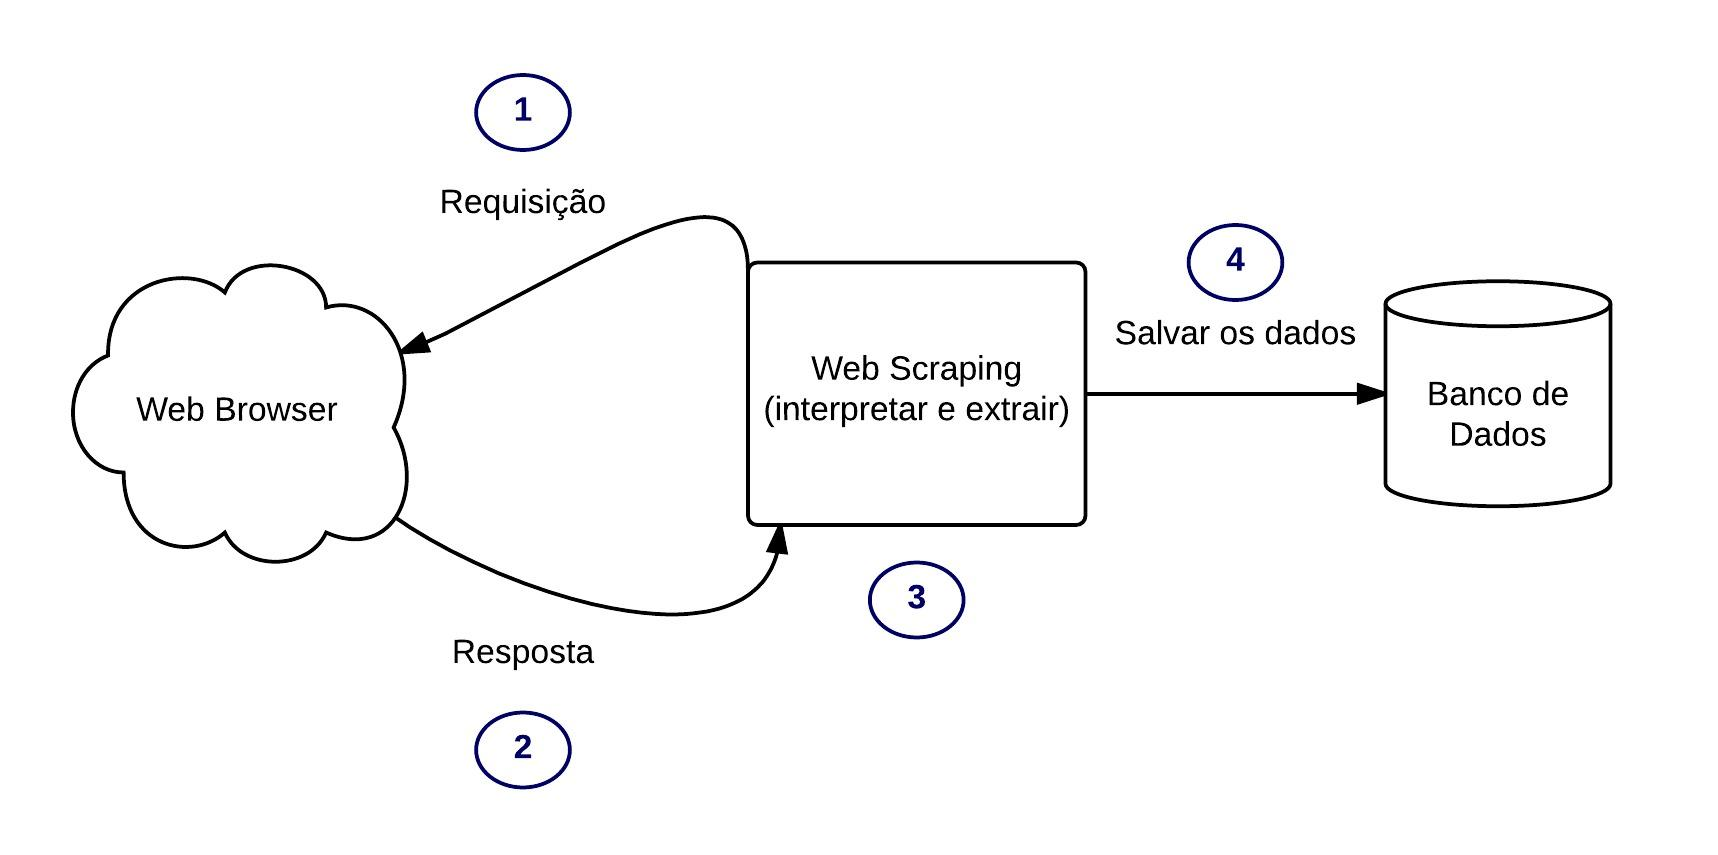
\includegraphics[width=\textwidth]{WebScraping}
  \caption[Figura Simples]{Arquitetura do Sistema de Coleta e Disponibilização dos Dados}
  \label{fig:01}
\end{figure}

Através de um coletor é possível arquiteturar e executar de forma lógica e escalável todo esse processo. Para que um coletor seja funcional é necessário que o mesmo seja capaz de interagir com páginas da Web, extrair a informação de interesse e estruturar e armazenar os dados para futuras consultas. Em geral, exemplos corriqueiros de coletores podem ser citados como os desenvolvidos pelo Google e Microsoft para atuar na procura por páginas da internet ou outros mais específicos para coleta de preços de produtos como os portais de agregadores como Bom de Faro, Buscapé dentre outros. Assim, como \citet{cavallo2010scraped}, o presente projeto de tese busca de forma inovadora para a economia brasileira, explorar preços coletados de sites de supermercados, farmácias, companhia de energia elétrica, lojas de varelo online, lojas de roupas e calçados, entre outros, e propõe o uso de um sistema de coleta como o apresentado a seguir. 

O sistema de coleta de preços está apresentado na Figura~\ref{fig:01}. O coletor recebe como entrada os templates dos sites que se deseja coletar e produz como resposta informações estruturadas com os atributos dos produtos. Para que o coletor seja capaz de realizar a tarefa de extração de informação, o mesmo deve apresentar os seguintes componentes: um componente centralizado capaz de ler instruções e aplicar regras para extração (1 - módulo coletor de dados); ter um conjunto de regras que descreva de forma não ambígua como realizar a coleta dos dados e os atributos de interesse (2 - templates dos webistes de supermercado, por exemplo); ter um banco de dados capaz de lidar com as características dos dados armazenados (3 - módulo de banco de dados); ter uma interface para facilitar o acesso aos dados por meio de outras aplicações ou sistemas web (4 - módulo de disponibilização da informação). Dessa forma, o coletor (1) é o centralizador do processo de coleta de dados, fazendo a interação com os templates (2), os webistes (A) e o módulo de banco de dados (3). Em resumo, o coletor através de um algoritmo inicia o processo de coleta carregando em uma lista os templates de coleta dos websites (2) e em seguida através de um processo iterativo visita o website, coleta os documentos de interesse e realiza a extração das informações indicadas pelo template. Ao final da coleta os dados são estruturados em um formato de documento denominado JSON e armazena-os em um banco de dados NoSQL adequado a essa estrutura de dados. O processo se repete para cada template até que todos os templates sejam avaliados. O algoritmo que descreve esse processo é apresentando em Algoritmo 1. Por fim, além da coleta em si, há um módulo para disponibilizar o acesso a informação coletada. Esse módulo (4) é responsável por permitir de forma segura e racional o uso dos dados coletados por diferentes sistemas e aplicações web existentes (C).

Segundo \citet{cavallo2010scraped}, preços coletados da internet possuem duas desvantagens: Primeiro, percentual menor de empresas disponibiliza seus produtos e preços na internet em comparação com as lojas físicas. Tal limitação pode ser minimizada ao longo do tempo com uma maior oferta de produtos e serviços na internet. Segundo, os preços coletados da internet não incluem informações sobre as quantidades vendidas o que impede de obter market share e estimativas de elasticidade.

Avaliações futuras precisarão ser feitas de forma que seja capaz explorar se os preços online e off-line se comportam similarmente. Preocupado com tal validação, \citet{cavallo2010scraped} fez pesquisa de preços nas lojas físicas dos supermercados utilizados para coleta de dados da internet. Desta forma, o autor examinou se os preços dos produtos nas lojas físicas eram similares aos preços nos sites. Uma importante característica é que um alto percentual de produtos vendidos nas lojas físicas também era comercializado nos sites em todos os países. O autor comparou os preços tanto em termo de nível quanto em tamanho e intervalo de tempo de alterações nos preços. Tal comportamento é muito importante para a avaliação de rigidez nos preços. Para tanto, o autor criou uma série de mudança de preços para cada produto que recebe valor 1 se o preço aumentou, 0 se o preço permaneceu constante e -1, caso contrário.  Assim, foi possível avaliar se os preços dos produtos nas lojas físicas são semelhantes em nível e em direção de mudança para cada produto e supermercado dos países avaliados por \citet{cavallo2010scraped}.

Não obstante, \citet{cavallo2010scraped} apresenta algumas vantagens dos preços coletados da internet que os fazem uma fonte única de informação para análise de rigidez nos preços. Primeiro, pode-se obter preços diários para os produtos e serviços e por conseguinte, reduzir medidas de erro em relação à frequência de cálculo da inflação, analisar promoções de produtos, controles e sincronização nos preços. Segundo, os dados estão disponíveis para vários países, com maior facilidade de acesso e possibilidade de comparação entre países. Terceiro, existem informações detalhadas sobre cada produto e não há substituições forçada de itens como ocorre em estatísticas oficiais de inflação. Por fim, preços coletados da internet estão viáveis em tempo real, sem qualquer atraso para acessá-los. Isto pode ser usado para providenciar estimativas de rigidez nos preços em tempo real.
  
\section*{ÍNDICE DE PREÇOS ONLINE}
  
Para calcular o índice de preços online que será comparado com o Índice Nacional de Preços ao Consumidor Amplo (IPCA) e Índice Nacional de Preços ao Consumidor (INPC) divulgados pelo Instituto Brasileiro de Geografia e Estatística (IBGE), utilizaremos a abordagem proposta por \citet{cavallo2010scraped}.
  
Assim, o índice de preços usa a combinação de dados online e as estruturas de ponderação oficiais do IBGE para as categorias da “cesta de mercadorias”\footnote[1]{Segundo o \citet{ibgemetodos} os índices constituem uma medida síntese de movimento de preços de um conjunto de bens e serviços, chamado “cesta de mercadorias”, representativo de um determinado grupo populacional, em certo período de tempo} de cada índice de inflação. Maiores detalhes sobre a metodologia de coleta e cálculo do IPCA e INPC podem ser obtidas no~\ref{ap1}. Dados diários serão utilizados para construir o índice de preços online o que é útil para observar padrões de curto prazo nos dados que ajudam a validar as informações online. 
  
O índice de preço online será calculado utilizando os preços de todos os produtos disponíveis para compra em cada site. Isto implica que a cesta de bens muda dinamicamente ao longo do tempo podendo um produto aparecer ou desaparecer da cesta a qualquer momento devido à disponibilidade ou indisponibilidade no site. Além disso, o número de preços por produto tende a ser muito maior o que os coletados usualmente pelos órgãos governamentais. 
Para construir o índice, mudanças de preço são calculadas em nível de produto, então as médias dentro das categorias usando média geométrica ponderada e finalmente agregado entre categorias com uma média aritmética ponderada. Em particular, o primeiro passo é obter a média geométrica ponderada das mudanças nos preços na categoria $j$ para cada dia $t$:

\begin{equation}\label{eq1}
R_{t,t-1}^{j}=\prod_{i}\left(\frac{p_{t}^{t}}{p_{t-1}^{i}}\right)^{\nicefrac{1}{n_{j,t}}}
\end{equation}

\noindent onde $p_{t}^{i}$ é o preço do bem $i$ no tempo $t$, $n_{j,t}$ é o número de produtos na categoria $j$ que estão presentes na amostra neste dia. 

O segundo passo é computar o índice em nível de categoria em $t$:

\begin{equation}\label{eq2}
I_{t}^{j}=R_{1,0}^{j}\ast{R}_{2,1}^{j}\ast{...}\ast{R}_{t,t-1}^{j}
\end{equation}

Finalmente, o índice de preços no tempo $t$ é a média aritmética ponderada de todos os índices das categorias:

\begin{equation}
IPO_{t}=\sum_{j}{\frac{w_{j}}{w}I_{t}^{j}} 
\end{equation}

\noindent onde $w^{j}$ é o peso oficial utilizado pelo IBGE para tal categoria e $W$ a soma de todos os pesos incluídos na amostra.

A classificação de produtos e pesos de categorias é uma das partes mais complexas deste processo. Nos dados originais, cada produto é atrelado à um endereço de web (URL) que corresponde à página onde o produto é localizado. 

\section*{RIGIDEZ DE PREÇOS}

 Diversas estatísticas poderão ser utilizadas para a análise da rigidez de preços coletados da internet, como por exemplo: frequência de produtos com alterações diarias e frequências de alta e baixa em relação ao total de alterações nos preços em um dia. Assim, teremos um parâmetro que reflete a probabilidade incondicional de mudança no preço de uma firma ao longo de um dado período de tempo. Porém, a análise da frequência apresenta uma visão parcial do comportamento dos preços e faz-se necessário avaliar o tamanho da mudança dos preços por meio do valor absoluto da alteração no preço de um determinado produto (tambéma o tamanho das mudanças positivas e negativas) e avaliação da sua distribuição de probabilidade. Desta forma, poder-se-a comparar o comportamento da inflação em determinadas regiões, municípios e estados em relação ao tamanho da mudança nos preços nestes locais. 
 
\citet{cavallo2010scraped} encontrou uma característica bimodal na distribuição do tamanho das alterações nos preços e uma forte queda da densidade das alterações próximo a 0\% em alguns países, o que é consistente com os modelos de custo de menu que mudanças muito pequenas não são ótimas na presença de custo de ajuste. Outro tipo de análise é a avaliação da assimetria na densidade das alterações que pode refletir maior quantidade de preços crescendo que diminuíndo. 
 
\subsection*{Análise de Sobrevida}

A análse de frequência ajudará na avaliação da rigidez de preços, mas ela sugere que a probabilidade de um preço se alterar é independente do tempo que uma mudança ocorre em relação à última alteração no preço. Ainda, a taxa de risco do preço se alterar é constante ao longo do tempo durante todo o período amostral. Embora esse método seja simples e efetivo para a comparação do grau de rigidez entre setores, regiões, cidades e países, um importante ponto reside sobre a forma da função risco. 

Para avaliar a função risco utilizaremos a Análise de Sobrevida assim como \citet{cavallo2010scraped}. Conforme \citet{colosimo2006analise}, em análise de sobrevivência, a variável resposta é, geralmente, o tempo até a ocorrência de um evento de interesse. Tal tempo é comumente conhecido como tempo de falha. Em medicina é comum o uso do método para a avaliação do tempo até a morte, transplante, doença, cura  entre outros. No contexto de preços, estamos interessados no tempo até o ajuste do preço. Assim, tanto o aparecimento do risco e o evento de falha ocorrem quando uma firma muda seus preços.  

A principal característica de dados de sobrevivência é a presença de censura que é a observação parcial da resposta. Isto se refere a situações em que por alguma razão, o acompanhamento do preço foi interrompido, seja porque a firma não vende mais um produto ou este não é produzido. A variável aleatória não-negativa $T$, usualmente contínua, que representa o tempo de falha, é geralmente especificada em análise de sobrevivência pela sua função de sobrevivência ou pela função de risco (tempo de falha). Estas duas funções são extensivamente usadas na análise de dados de sobrevivência. 

Segundo \citet{colosimo2006analise}, a função de sobrevivência é definida como a probabilidade de uma observação não falhar até um certo tempo $t$, ou seja, a probabilidade de uma observação sobreviver (preço não se alterar) ao tempo $t$. Por outro lado, se $T$ é a variável aleatória que mede a duração do preço, com função densidade $f\left(t\right)$ e densidade acumulada $F\left(t\right)$, o risco $h\left(t\right)$ é a probabilidade limite de que a mudança no preço ocorra em $t$, condicional ao preço não se alterar até este momento. 

\begin{equation}
h\left(t\right)=\lim_{\Delta t\rightarrow 0}{\frac{Pr\left(t<T<t+\Delta t|t<T\right)}{\Delta t}=\frac{f\left(t\right)}{1-F\left(t\right)}} 
\end{equation}

Esta função risco mede o risco instantâneo de um preço se alterar, condicionado à sobrevida. Podemos adicionar todas as taxas de risco ao longo do tempo e obter o risco total de um preço alterar acumulado até o tempo $t$. Isto é representado pelo função risco acumulado, $H(t)$:

\begin{equation}
H\left(t\right)=\int_{0}^{t}{h\left(u\right)du=-\ln{\left(1-F\left(t\right)\right)}} 
\end{equation}

$H(t)$ é um aumento, função ilimitada de $t$, que acumula a probabilidade condicional do preço mudar ao longo do tempo. No contexto de repetidas "falhas" (preço se alterar), ela pode ser interpretada com o número esperado de ajustamento nos preços de $0$ à $t$. O risco acumulado recebe grande atenção na Análise de Sobrevida porque ele é mais fácil de estimar do que a função risco sózinha. 

Para estimar $H(t)$ e $h(t)$ empiricamente, usaremos conforme \citet{cavallo2010scraped} uma abordagem não paramétrica dada por Nelson (1972) e Aalen (1978), que não requer hipóteses de distribuição de probabilidade. Métodos semi-paramétricos como o modelo Cox podem ser utilizados futuramente uma vez que permitem a incorporação de variáveis explicativas e a consideração da heterogeneidade não observável em nível de categoria de preços. Uma estimativa simples da função risco acumulado, $H(t)$, é dado por:

\begin{equation}
\hat{H}\left(t\right)=\sum_{j|{t}_{j}\le t}{\frac{{c}_{j}}{{n}_{j}}} 
\end{equation}

\noindent onde ${c}_{j}$ é o número de preços que mudaram em ${t}_{j}$ e ${n}_{j}$ é o número de preços sob risco em ${t}_{j}$, ou seja, os preços que não alteraram e não foram censurados até o instante imediatamente anterior a $t_{j}$. O passo incremental $\frac{{c}_{j}}{{n}_{j}}$ é uma estimativa para a probabilidade do preço mudar em ${t}_{j}$, levando em consideração apenas aqueles preços que sobreviveram até este ponto no tempo. 

Para obter a função risco suavizada $\hat{h}\left(t\right)$, pode-se usar a seguinte equação:

\begin{equation}
\hat{h}\left(t \right)=\frac{1}{b}\sum_{j\epsilon D}{K}\left(\frac{t-{t}_{j}}{b}\right)\Delta \hat {H}\left({t}_{j}\right) 
\end{equation}

\noindent onde $K$ é um kernel com densidade simétrica, $b$ é a \emph{bandwidth} de suavização e $D$ é o conjunto de vezes com mudança de preços. 


% \SweaveInput{final.Rnw}

% Formato da bibliografia
\bibliographystyle{apalike}

% Arquivo .bib
\bibliography{projeto}

% Apêndice(s)
\appendix

\chapter{METODOLOGIA IBGE}\label{ap1}

O Sistema Nacional de Preços ao Consumidor (SNIPC) efetua a produção e sistemática de índices de preços ao consumidor tendo como unidade de coleta estabelecimentos comerciais e de prestação de serviços, concessionária de serviços públicos e domicílios (para levantamento de aluguel e condomínio). O sistema abrange as regiões metropolitanas do Rio de Janeiro, Porto Alegre, Belo Horizonte, Recife, São Paulo, Belém, Fortaleza, Salvador e Curitiba, além do Distrito Federal e do município de Goiânia. A partir de janeiro de 2014, o SNIPC passou a incorporar a Regiâo Metropolitana de Vitória/ES e o município de Campo Grande/MS. 

As motivações para criação do Índice Nacional de Preços ao Consumidor Amplo (IPCA) e Índice Nacional de Preços ao Consumidor (INPC) foram a obtenção de medida geral de inflação e a indexação salarial, respectivamente.

% A partir de Janeiro de 2012, o IPCA passou a ser calculado com base nos valores de despesa obtidos na Pesquisa de Orçamentos Familiares (POF 2008-2009) . A POF é realizada a cada cinco anos pelo IBGE em todo o território brasileiro o que permite atualizar os pesos dos produtos e serviços nos orçamentos das famílias. Na tabela abaixo, os pesos antigos e atuais de cada produto e serviço.
% 
% 
% \begin{table}[h]
% \centering
% \begin{tabular}{lcc}
% \hline
% \multicolumn{3}{c}{PESO POR GRUPO DE PRODUTO E SERVIÇO} \\ \hline
% \multicolumn{1}{c}{TIPO DE GASTO} & \begin{tabular}[c]{@{}c@{}}ATÉ 31.12.2011\\ (\%)\end{tabular} & \begin{tabular}[c]{@{}c@{}}A PARTIR 01.01.2012\\ (\%)\end{tabular}  \\ \hline
% Alimentação e Bebidas     & 23,46 & 23,12  \\
% Transportes               & 18,69 & 20,54  \\
% Habitação                 & 13,25 & 14,62  \\
% Saúde e cuidados pessoais & 10,76 & 11,09  \\
% Despesas Pessoais         & 10,54 & 9,94   \\
% Vestuário                 & 6,94  & 6,67   \\
% Comunicação               & 5,25  & 4,96   \\
% Artigos de Residência     & 3,90  & 4,69   \\
% Educação                  & 7,21  & 4,37   \\
% \textbf{TOTAL}            & \textbf{100} & \textbf{100} \\ \hline                                                     
% \end{tabular}
% \caption{Pesos por tipo de gasto}
% \label{table:03}
% \end{table}

As etapas para a construção dos índices de preços são elencadas abaixo. Para maiores detalhes, consultar \citet{ibgemetodos}.

\begin{enumerate}
  \item Definição da população objetivo: 
  \begin{enumerate} 
    \item Para o INPC são a famílias residentes nas áreas urbanas das regiões de abrangência do SNIPC com rendimentos de 1 a 6 salários-mínimos e cujos chefes são assalariados; 
    \item Para o IPCA, as familias residentes nas áreas urbanas das regiões de abrangência do SNIPC com rendimentos de 1 a 40 salários-mínimos, qualquer que seja a fonte de rendimentos.
  \end{enumerate}
  \item Obter estruturas de ponderação: O conjunto de bens e serviços representativos do consumo dos grupos e os valores de despesa que lhes são associados. 
  \begin{enumerate}
    \item Pode ser diferente para uma determinada população-objetivo;
    \item São resultado da consolidação dos orçamentos familiares levantados pela POF;
    \item São montadas de forma que categorias de consumo de mesma natureza fiquem juntas. Hierarquicamente \footnote[2]{Por exemplo, Laranja-pera é um subitem do item "Frutas" que conjuntamente com outros itens formam o subgrupo "Alimentação no Domicílio", o qual, unido ao subgrupo "Alimentação Fora do Domicílio" compõe o grupo "Alimentação e Bebidas". Retirado de \citet{ibgemetodos}}: 
    \begin{enumerate}
      \item Grupo
      \item Subgrupo
      \item Item
      \item Subitem
    \end{enumerate}
  \end{enumerate}
  \item Cálcular os Pesos:
  \begin{enumerate}
    \item Anualisar os valores de despesa com consumo oriúndas da POF que são coletados em diferentes períodos de referência;
    \item Colocar as despesas anuais em preços constantes de 15 de janeiro de 2009;
    \item Somar para cada subitem, despesas das familias pertencentes à população-objetivo;
    \item A razão da soma anterior e a despesa total de todas as familias da região em questão gera o índice.
  \end{enumerate}
  \item Definir estruturas de consumo: A partir da participação dos subitens, define-se quais permanecerão para o cálculo do índice. Para tanto, utiliza-se o seguinte critério:
    \begin{enumerate}
    \item subitens com participação igual ou superior a 0,07\% fazem parte das estruturas;
    \item subitens com participação inferior a 0,01\% em hipótese alguma fazem parte das estruturas;
    \item subitens com ponderação igual ou superior a 0,01\% e inferior a 0,07\% podem fazer parte para assegurar que o item do qual fazem parte tenha cobertura de 70\% dos gastos realizados com os componentes do item.
    \end{enumerate}
  \item Cadastrar informantes: Por meio da Pesquisa de Locais de Compra (PLC) faz-se o cadastro dos estabelecimentos.
  \item Cadastrar produtos: Por meio da Pesquisa de Especificação de Produtos e Serviços (PEPS) obtém-se os produtos.
  \item Coletar preços: Tarefa contínua, realizada mensalmente, nas áreas de cobertura da pesquisa, ao longo do mês. Para viabilizá-la existem pesquisadores de campo dedicados à coleta de informações necessárias à produção dos índices. Questionário eletrônico de coleta instalado em computador de mão, no qual estão descritas as características dos produtos ou serviços nele investigados.
\end{enumerate}

A tabela~\ref{table:01}, apresenta um resumo das fontes de informações relevantes para os índices de preços: Pesquisa de Orçamentos Familiares (POF), Pesquisa de Locais de Compra (PLC) e Pesquisa de Espicificação de Produtos e Serviços (PEPS).

\begin{table}[h]
\centering
\begin{tabular}{lc}
\hline
\multicolumn{2}{c}{PESQUISAS BÁSICAS}                                            \\ \hline
POF & Fornece as estruturas de ponderação para cada grupo de bens e serviços).   \\
PLC & Fornece o cadastro de informantes da pesquisa que tem manutenção constante.\\ 
PEPS & Fornece o cadastro de produtos e serviços a serem pesquisados.            \\ \hline
\end{tabular}
\caption{Principais Pesquisas Utilizadas na Metodologia}
\label{table:01}
\end{table}

Por fim, temos a metodologia de cálculo dos índices de preços. Sinteticamente, partindo-se de milhares de preços coletados mensalmente, obtêm-se no primeiro processo-síntese, as estimativas dos movimentos de preços referentes a cada produto pesquisado. Estes resultados são agregados por uma fórmula elementar de cálculo e geram a estimativa para variação de preços de cada subitem; essas estimativas, por sua vez, por outro processo agregativo, produzem os índices referentes a itens, que, por fim, geram os índices regionais e nacional mensais de cada população-objetivo.

\section*{Cálculo no nível de produto}

Primeiro, calcula-se mensalmente o relativo de preços referentes a dois meses e temos a estimativa da variação mensal dos preços do produto $j$, ou relativo do produto $j$, conforme:

\begin{equation}\label{eq3}
{R}_{t-1,t}^{j}=\frac{{\overline{P}}_{t}^{j}}{{\overline{P}}_{t-1}^{j}}=\frac{\frac{1}{{n}_{t}}\sum_{L=1}^{{n}_{t}}{{p}_{t}^{j,L}}}{\frac{1}{{n}_{t-1}}\sum_{L=1}^{{n}_{t-1}}{{p}_{t-1}^{j,L}}} 
\end{equation}

\noindent onde ${R}_{t-1,t}^{j}$ é a medida da variação de preços do produto $j$ entre os meses $t-1$ e $t$, ${\overline{P}}_{t}^{j}$ e ${\overline{P}}_{t-1}^{j}$ os preços médio do produto $j$ nos meses $t$ e $t-1$, respectivamente, assim como ${p}_{t}^{j,L}$ e ${p}_{t-1}^{j,L}$ são os preços do produto $j$ no local $L$ nos meses $t$e $t-1$. Por fim, ${n}_{t}$ e ${n}_{t-1}$ são os números de locais que compõem a amostra do produto nos meses $t$ e $t-1$.

Por conseguinte, o próximo passo é a agregação no nível de subitem. Para tanto, calcula-se a média geométrica dos resultados obtidos para cada produto que compõe o subitem. Assim, 

\begin{equation}\label{eq4}
{R}_{t-1,t}^{k}=\sqrt[{m}_{k}]{\prod_{j=1}^{{m}_{k}}{{R}_{t-1,t}^{j}}} 
\end{equation}

\noindent onde ${R}_{t-1,t}^{k}$ é a variação média de preços entre os meses $t-1$ e $t$ dos produtos que compõem o subitem $k$, ${R}_{t-1,t}^{j}$ é a variação do preço do produto $j$ entre os meses $t-1$ e $t$ (fórmula~\ref{eq3) e $m_{k}$ é o número de produtos do subitem $k$. Como observa-se da equação~\ref{eq4}, todos os produtos participam do resultado do subitem com a mesma ponderação.

No que diz respeito aos resultados ao longo do tempo, evidencia-se a importância de manter-se o painel de produtos fixos, a exemplo do que ocorre com o painel de locais, sob pena de incorporar falsas variações de preços. Desta forma, o IBGE imputa o preço de um produto para determinado local ou subitem. Para maiores informações de como é feito esse processo, consultar \citet{ibgemetodos}.

\section*{Cálculo no nível de item}

Usa-se a fórmula de Laspeyres que expressa a razão entre o gasto efetuado no momento $t$, necessário para consumir as mesmas quantidades do momento $0$, e o gasto efetuado no momento $0$. A fórmula~\ref{eq5} representa o índice:

\begin{equation}\label{eq5}
{L}_{0,t}=\sum_{i=1}^{n}{\left(\frac{{p}_{0}^{i}{q}_{0}^{i}}{\sum_{j=1}^{n}{{p}_{0}^{j}{q}_{0}^{j}}}\right)}\left(\frac{{p}_{t}^{i}}{{p}_{0}^{i}}\right) 
\end{equation}

\noindent onde $\frac{{p}_{t}^{i}}{{p}_{0}^{i}}=R_{0,t}^{i}$ é o estimador da variação de preços do subitem $i$ entre os momentos $0$ e $t$ e $\frac{{p}_{0}^{i}{q}_{0}^{i}}{\sum_{j=1}^{n}{{p}_{0}^{j}{q}_{0}^{j}}}=W_{0}^{i}$ é o peso do subitem $i$ obtido a partir da POF. Observe-se que tanto $R_{0,t}^{i}$ como $W_{0}^{i}$ referem-se, na prática, a pequenos agregados de produtos. Para se conhecer a variação de preços do item $m$ para uma determinada área e faixa de rendimento em ciclos mensais utiliza-se a fórmula~\ref{eq6}.

\begin{equation}\label{eq6}
{I}_{t-1,t}^{m}=\frac{\sum_{i=1}^{n}{{W}_{t-1}^{i}{R}_{t-1,t}^{i}}}{\sum_{i=1}^{n}{{W}_{t-1}^{i}}} 
\end{equation}

\noindent onde ${I}_{t-1,t}^{m}$ é o índice do item $m$ entre os meses $t-1$ e $t$, ${W}_{t-1}^{i}$ é o peso do subitem $i$ em $t-1$ e ${R}_{t-1,t}^{i}$ é o relativo do subitem $i$ entre $t-1$ e $t$. Além disso, o peso ${W}_{t-1}^{i}$ a partir de $t=2$ é dado por:

\begin{equation}\label{eq7}
{W}_{t-1}^{i}={W}_{0}^{i}\prod_{j=0}^{t-2}{\frac{{R}_{j,j+1}^{i}}{{I}_{j,j+1}}} 
\end{equation}

\noindent onde ${W}_{0}^{i}$ é o peso do subitem $i$ obtido a partir da POF, ${R}_{j,j+1}^{i}$ é o relativo do subitem $i$ entre os meses $j$ e $j+1$ e ${I}_{j,j+1}$ é o resultado do índice geral entre os meses $j$ e $j+1$.

\section*{Cálculo dos índices regionais}

O resultado mensal para a área $A$ e população-objetivo $F$ é dado por:

\begin{equation}\label{eq8}
{IPC}_{t-1,t}^{A,F}=\sum_{m}^{M}{{W}_{t-1}^{m}{I}_{t-1,t}^{m}} 
\end{equation}

\noindent onde ${I}_{t-1,t}^{m}$ é o índice do item $m$ obtido conforme a equação~\ref{eq6} e ${W}_{t-1}^{m}$ corresponde ao peso de cada item e é obtido somando-se os pesos no período $t-1$ por meio da equação~\ref{eq7} utilizando todos os subitens que compõem o respectivo item $m$.

\section*{Cálculo dos índices nacionais}

Os índices nacionais são obtidos a partir dos índices regionais. O método empregado para obtenção dos índices nacionais consiste no cálculo de uma média aritmética ponderada dos índices regionais mensais, conforme:

\begin{equation}\label{eq9}
{INPC}_{t-1,t}=\sum_{A=1}^{11}{{W}^{A,F}{IPC}_{t-1,t}^{A,F}}
\end{equation}

\noindent onde ${INPC}_{t-1,t}$ é o índice nacional referente à variação de preços entre os meses $t-1$ e $t$, ${IPC}_{t-1,t}^{A,F}$ é o índice da área $A$, população-objetivo $F$, obtido via~\ref{eq8}. Além disso, ${W}^{A,F}$ é o peso da área $A$, população-objetivo $F$. Na mais recente atualização, tendo como fonte a POF 2008-2009, os pesos das regiões foram obtidos com base nas estimativas da população urbana para os estados, Grandes Regiões e Brasil. A tabela~\ref{table:02}, apresenta os índices regionais antes e após a alteração. 

\begin{table}[h]
\centering
\begin{tabular}{lll}
\hline
\multicolumn{1}{l|}{Regiões} & \multicolumn{1}{l|}{IPCA} & INPC  \\ \hline
Belém                      & 4,65                      & 7,03  \\
Fortaleza                  & 3,49                      & 6,61  \\
Recife                     & 5,05                      & 7,17  \\
Salvador                   & 7,35                      & 10,67 \\
Belo Horizonte             & 10,86                     & 10,60 \\
Vitória                    & 1,78                      & 1,83  \\
Rio de Janeiro             & 12,06                     & 9,51  \\
São Paulo                  & 30,67                     & 24,24 \\
Curitiva                   & 7,79                      & 7,29  \\
Porto Alegre               & 8,40                      & 7,38  \\
Campo Grande               & 1,51                      & 1,64  \\
Goiânia                    & 3,59                      & 4,15  \\
Brasília                   & 2,80                      & 1,88  \\ \hline
\end{tabular}
\caption{Participação do índice regional no agregado nacional}
\label{table:02}
\end{table}
\appendix

\chapter{ARQUITETURA E EXEMPLO DE COLETA}\label{ap2}

\begin{Schunk}
\begin{Sinput}
> library(devtools)